
%%%%%%%%%%%%%%%%%%%%%%% file typeinst.tex %%%%%%%%%%%%%%%%%%%%%%%%%
%
% This is the LaTeX source for the instructions to authors using
% the LaTeX document class 'llncs.cls' for contributions to
% the Lecture Notes in Computer Sciences series.
% http://www.springer.com/lncs       Springer Heidelberg 2006/05/04
%
% It may be used as a template for your own input - copy it
% to a new file with a new name and use it as the basis
% for your article.
%
% NB: the document class 'llncs' has its own and detailed documentation, see
% ftp://ftp.springer.de/data/pubftp/pub/tex/latex/llncs/latex2e/llncsdoc.pdf
%
%%%%%%%%%%%%%%%%%%%%%%%%%%%%%%%%%%%%%%%%%%%%%%%%%%%%%%%%%%%%%%%%%%%


\documentclass[runningheads,a4paper]{llncs}

\usepackage{amssymb}
\setcounter{tocdepth}{3}
\usepackage{graphicx}
\usepackage{longtable}
\usepackage{url}  
\newcommand{\keywords}[1]{\par\addvspace\baselineskip
\noindent\keywordname\enspace\ignorespaces#1}

\usepackage{nameref}
\begin{document}

\mainmatter  % start of an individual contribution

% first the title is needed
\title{DAT530\\Discrete Simulation and Performance Analysis\\Final Project\\Solitaire game strategy}

% a short form should be given in case it is too long for the running head
\titlerunning{DAT530 - Final Project}


\author{Racin W. Nygaard}%

%
\authorrunning{DAT530 - Final Project - Solitaire game strategy}
% (feature abused for this document to repeat the title also on left hand pages)

% the affiliations are given next; don't give your e-mail address
% unless you accept that it will be published
\institute{Universitetet i Stavanger}

%
% NB: a more complex sample for affiliations and the mapping to the
% corresponding authors can be found in the file "llncs.dem"
% (search for the string "\mainmatter" where a contribution starts).
% "llncs.dem" accompanies the document class "llncs.cls".
%

\toctitle{Solitaire game strategy}
\tocauthor{Report}
\maketitle


\begin{abstract}
SKRIV DETTE TIL SLUTT!

\end{abstract}


\section{Introduction}
This project aims to study the popular card game, Solitaire[Site]. Solitaire is bundled with most Windows[Site] installations, as well as being available for free on several sources. It is also easy to play the game with a physical card deck. A detailed explaination of the games rules can be found in the next chapter, Solitaire Rules[REF]
\newline
Since the game utilizes all 52 cards of the deck, the number of possible initial game states is 52!, which is a very high number. A large number of these inital game states can be merged, as they offer no difference in the difficulty to solve. Some of these intial states are unsolvable, but even given a solvable game state, one often find oneself in an unsolvable game state, due to certain actions in the game are non-reversible,. There has been attempts to find the distribution of solvable and unsolvable initial game states [ref]. This is roughly 75 percent are solvable, however the study also shows that only 35 percent of the games are won by an experienced player.
\newline
This project contains a complete model of the game, a GUI to play the game, and a basic bot to simulate user actions. 

\subsection{Solitaire Rules}

Finite State Machine ?


\section{Method and Design}
\label{sec:2_method_and_design}
\subsection{Naming Policy}
%\begin{table}
%	\caption{Places}
%	\begin{tabular}{|l|l|l|l|}
%		\hline
%		 & Name & Module & Usage \\
%		\hline
%		9  & tFPe\_Clubs\_Add         &  &  \\ \hline
%		10 & tFPe\_Clubs\_Move        &  &  \\ \hline
%		11 & tFPe\_Clubs\_Out         &  &  \\ \hline
%		12 & tFPe\_Diamonds\_Add      &  &  \\ \hline
%		13 & tFPe\_Diamonds\_Move     &  &  \\ \hline
%		14 & tFPe\_Diamonds\_Out      &  &  \\ \hline
%		15 & tFPe\_Hearts\_Add        &  &  \\ \hline
%		16 & tFPe\_Hearts\_Move       &  &  \\ \hline
%		17 & tFPe\_Hearts\_Out        &  &  \\ \hline
%		18 & tFPe\_Spades\_Add        &  &  \\ \hline
%		19 & tFPe\_Spades\_Move       &  &  \\ \hline
%		20 & tFPe\_Spades\_Out        &  &  \\ \hline
%		21 & tMC\_DP\_Move\_Siphon    &  &  \\ \hline
%		22 & tMC\_FP\_Move\_Siphon    &  &  \\ \hline
%		23 & tMC\_Out\_Buffer\_Siphon &  &  \\ \hline
%		24 & tMC\_TP\_Move\_Siphon    &  &  \\ \hline
%		25 & tMC\_TP\_Turn\_Siphon    &  &  \\ \hline
%		26 & tPBe\_DP\_Move           &  &  \\ \hline
%		27 & tPBe\_DP\_Turn           &  &  \\ \hline
%		28 & tPBe\_FP\_Move           &  &  \\ \hline
%		29 & tPBe\_TP\_Move           &  &  \\ \hline
%		30 & tPBe\_TP\_Turn           &  &  \\ \hline
%		31 & tPBi\_Gen                &  &  \\ \hline
%		32 & tPBi\_Siphon             &  &  \\ \hline
%		33 & tPe\_DP\_Move            &  &  \\ \hline
%		34 & tPe\_DP\_Turn            &  &  \\ \hline
%		35 & tPe\_FP\_Clubs\_Move     &  &  \\ \hline
%		36 & tPe\_FP\_Diamonds\_Move  &  &  \\ \hline
%		37 & tPe\_FP\_Hearts\_Move    &  &  \\ \hline
%		38 & tPe\_FP\_Spades\_Move    &  &  \\ \hline
%		39 & tPe\_TP\_1\_Move         &  &  \\ \hline
%		40 & tPe\_TP\_1\_Turn         &  &  \\ \hline
%		41 & tPe\_TP\_2\_Move         &  &  \\ \hline
%		42 & tPe\_TP\_2\_Turn         &  &  \\ \hline
%		43 & tPe\_TP\_3\_Move         &  &  \\ \hline
%		44 & tPe\_TP\_3\_Turn         &  &  \\ \hline
%		45 & tPe\_TP\_4\_Move         &  &  \\ \hline
%		46 & tPe\_TP\_4\_Turn         &  &  \\ \hline
%		47 & tPe\_TP\_5\_Move         &  &  \\ \hline
%		48 & tPe\_TP\_5\_Turn         &  &  \\ \hline
%		49 & tPe\_TP\_6\_Move         &  &  \\ \hline
%		50 & tPe\_TP\_6\_Turn         &  &  \\ \hline
%		51 & tPe\_TP\_7\_Move         &  &  \\ \hline
%		52 & tPe\_TP\_7\_Turn         &  &  \\ \hline
%		53 & tTPe\_1\_Add\_FaceDown   &  &  \\ \hline
%		54 & tTPe\_1\_Add\_FaceUp     &  &  \\ \hline
%		55 & tTPe\_1\_Move            &  &  \\ \hline
%		56 & tTPe\_1\_Out             &  &  \\ \hline
%		57 & tTPe\_1\_Turn            &  &  \\ \hline
%		58 & tTPe\_2\_Add\_FaceDown   &  &  \\ \hline
%		59 & tTPe\_2\_Add\_FaceUp     &  &  \\ \hline
%		60 & tTPe\_2\_Move            &  &  \\ \hline
%		61 & tTPe\_2\_Out             &  &  \\ \hline
%		62 & tTPe\_2\_Turn            &  &  \\ \hline
%		63 & tTPe\_3\_Add\_FaceDown   &  &  \\ \hline
%		64 & tTPe\_3\_Add\_FaceUp     &  &  \\ \hline
%		65 & tTPe\_3\_Move            &  &  \\ \hline
%		66 & tTPe\_3\_Out             &  &  \\ \hline
%		67 & tTPe\_3\_Turn            &  &  \\ \hline
%		68 & tTPe\_4\_Add\_FaceDown   &  &  \\ \hline
%		69 & tTPe\_4\_Add\_FaceUp     &  &  \\ \hline
%		70 & tTPe\_4\_Move            &  &  \\ \hline
%		71 & tTPe\_4\_Out             &  &  \\ \hline
%		72 & tTPe\_4\_Turn            &  &  \\ \hline
%		73 & tTPe\_5\_Add\_FaceDown   &  &  \\ \hline
%		74 & tTPe\_5\_Add\_FaceUp     &  &  \\ \hline
%		75 & tTPe\_5\_Move            &  &  \\ \hline
%		76 & tTPe\_5\_Out             &  &  \\ \hline
%		77 & tTPe\_5\_Turn            &  &  \\ \hline
%		78 & tTPe\_6\_Add\_FaceDown   &  &  \\ \hline
%		79 & tTPe\_6\_Add\_FaceUp     &  &  \\ \hline
%		80 & tTPe\_6\_Move            &  &  \\ \hline
%		81 & tTPe\_6\_Out             &  &  \\ \hline
%		82 & tTPe\_6\_Turn            &  &  \\ \hline
%		83 & tTPe\_7\_Add\_FaceDown   &  &  \\ \hline
%		84 & tTPe\_7\_Add\_FaceUp     &  &  \\ \hline
%		85 & tTPe\_7\_Move            &  &  \\ \hline
%		86 & tTPe\_7\_Out             &  &  \\ \hline
%		87 & tTPe\_7\_Turn            &  &  \\ \hline
%		88 & tTPi\_1\_Move\_Multiple  &  &  \\ \hline
%		89 & tTPi\_2\_Move\_Multiple  &  &  \\ \hline
%		90 & tTPi\_3\_Move\_Multiple  &  &  \\ \hline
%		91 & tTPi\_4\_Move\_Multiple  &  &  \\ \hline
%		92 & tTPi\_5\_Move\_Multiple  &  &  \\ \hline
%		93 & tTPi\_6\_Move\_Multiple  &  &  \\ \hline
%		94 & tTPi\_7\_Move\_Multiple  &  &  \\ \hline
%	\end{tabular}
%\end{table}
%\begin{table}
%	\caption{Places used in Draw Pile}
%	\begin{tabular}{|l|l|l|}
%		\hline
%		& Name & Description \\
%		\hline
%		7  & pFP\_Clubs\_Move          &  \\ \hline
%		8  & pFP\_Clubs\_Pile          &  \\ \hline
%		9  & pFP\_Diamonds\_Move       &  \\ \hline
%		10 & pFP\_Diamonds\_Pile       &  \\ \hline
%		11 & pFP\_Hearts\_Move         &  \\ \hline
%		12 & pFP\_Hearts\_Pile         &  \\ \hline
%		13 & pFP\_Spades\_Move         &  \\ \hline
%		14 & pFP\_Spades\_Pile         &  \\ \hline
%		15 & pMC\_DP\_Move             &  \\ \hline
%		16 & pMC\_DP\_Turn             &  \\ \hline
%		17 & pMC\_FP\_Move             &  \\ \hline
%		18 & pMC\_Out\_Buffer          &  \\ \hline
%		19 & pMC\_TP\_Move             &  \\ \hline
%		20 & pMC\_TP\_Turn             &  \\ \hline
%		21 & pPB\_Cmd                  &  \\ \hline
%		22 & pTP\_1\_FaceDown\_Pile    &  \\ \hline
%		23 & pTP\_1\_FaceUp\_Pile      &  \\ \hline
%		24 & pTP\_1\_Move              &  \\ \hline
%		25 & pTP\_2\_FaceDown\_Pile    &  \\ \hline
%		26 & pTP\_2\_FaceUp\_Pile      &  \\ \hline
%		27 & pTP\_2\_Move              &  \\ \hline
%		28 & pTP\_3\_FaceDown\_Pile    &  \\ \hline
%		29 & pTP\_3\_FaceUp\_Pile      &  \\ \hline
%		30 & pTP\_3\_Move              &  \\ \hline
%		31 & pTP\_4\_FaceDown\_Pile    &  \\ \hline
%		32 & pTP\_4\_FaceUp\_Pile      &  \\ \hline
%		33 & pTP\_4\_Move              &  \\ \hline
%		34 & pTP\_5\_FaceDown\_Pile    &  \\ \hline
%		35 & pTP\_5\_FaceUp\_Pile      &  \\ \hline
%		36 & pTP\_5\_Move              &  \\ \hline
%		37 & pTP\_6\_FaceDown\_Pile    &  \\ \hline
%		38 & pTP\_6\_FaceUp\_Pile      &  \\ \hline
%		39 & pTP\_6\_Move              &  \\ \hline
%		40 & pTP\_7\_FaceDown\_Pile    &  \\ \hline
%		41 & pTP\_7\_FaceUp\_Pile      &  \\ \hline
%		42 & pTP\_7\_Move              &  \\ \hline
%	\end{tabular}
%\end{table}
\subsection{Overall Design}
\begin{center} % Left, Bottom, Right, Top
	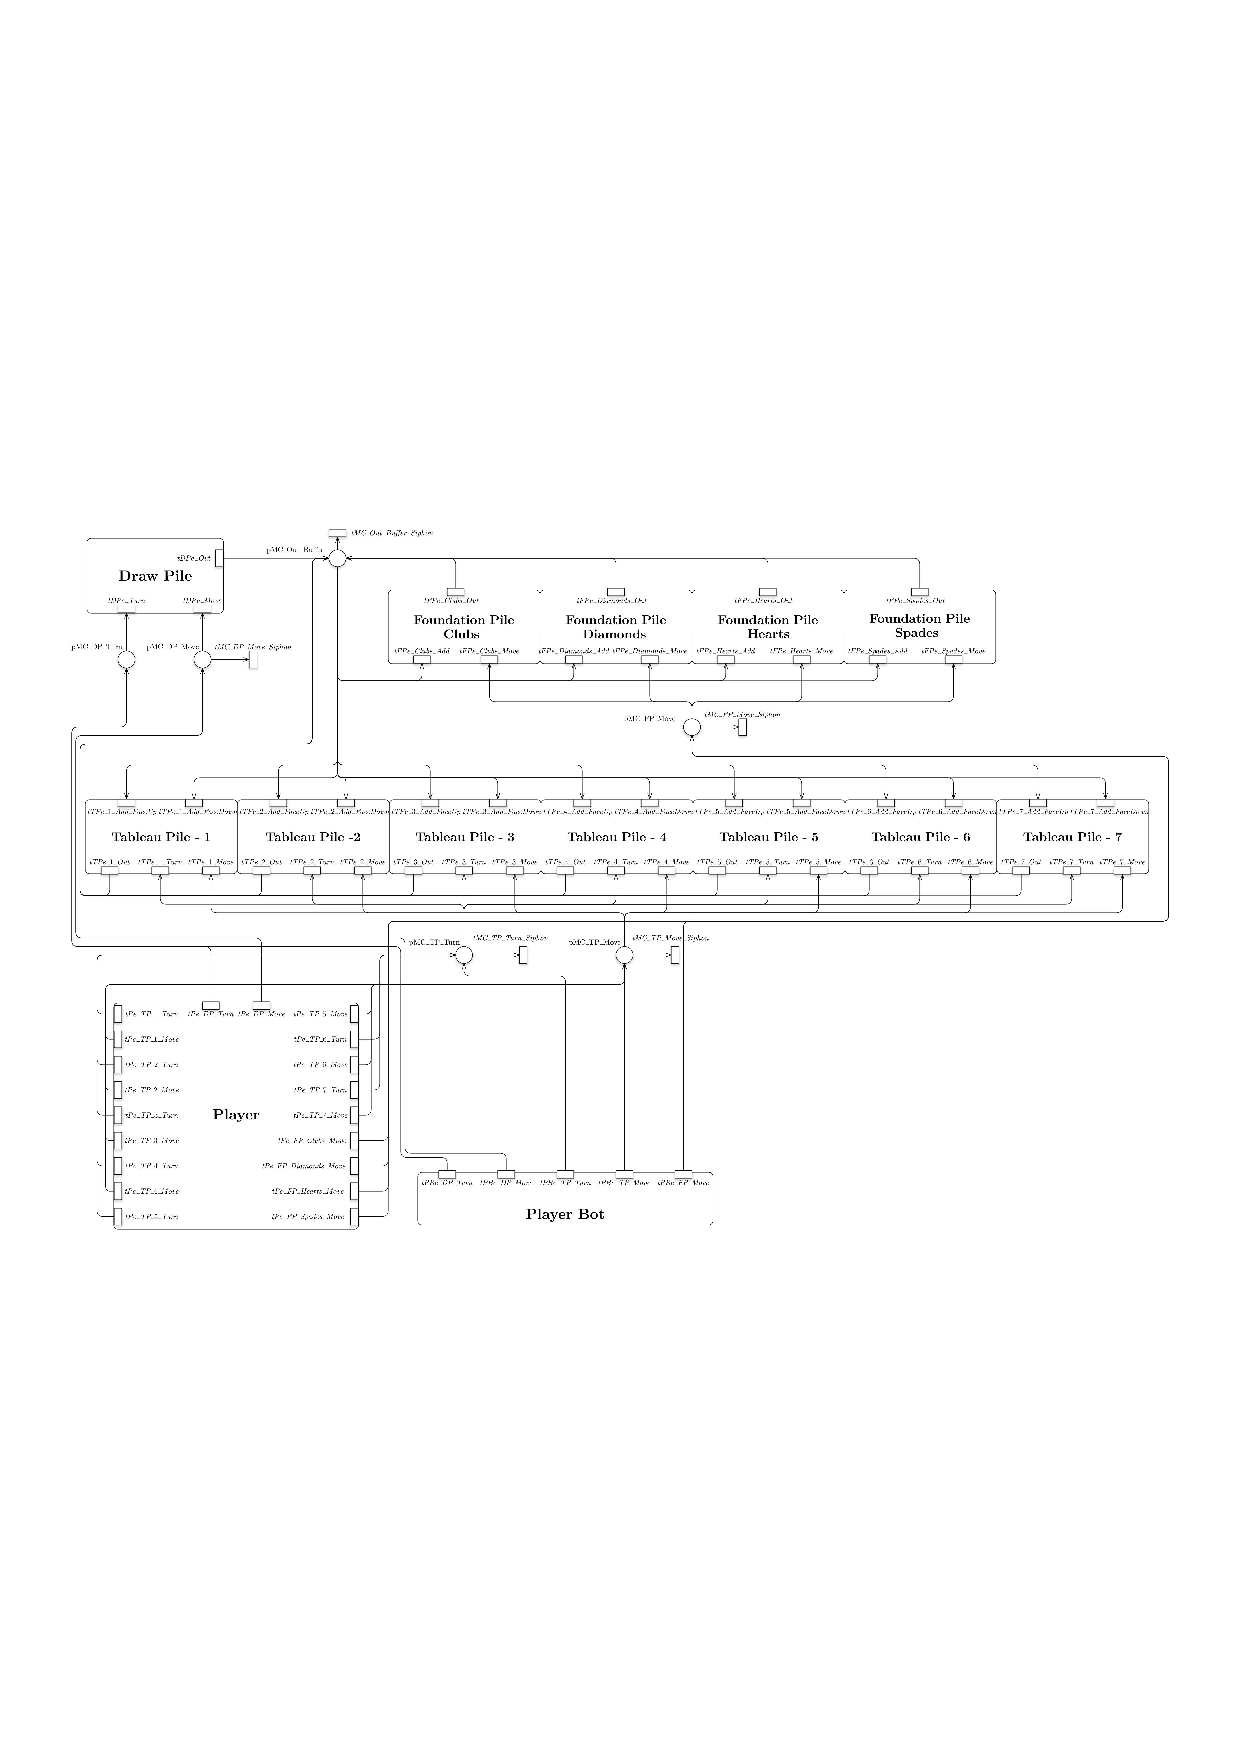
\includegraphics[trim=180 250 160 270]{images/overallViewPdf}
\end{center}
\newline
\begin{center} % Left, Bottom, Right, Top
	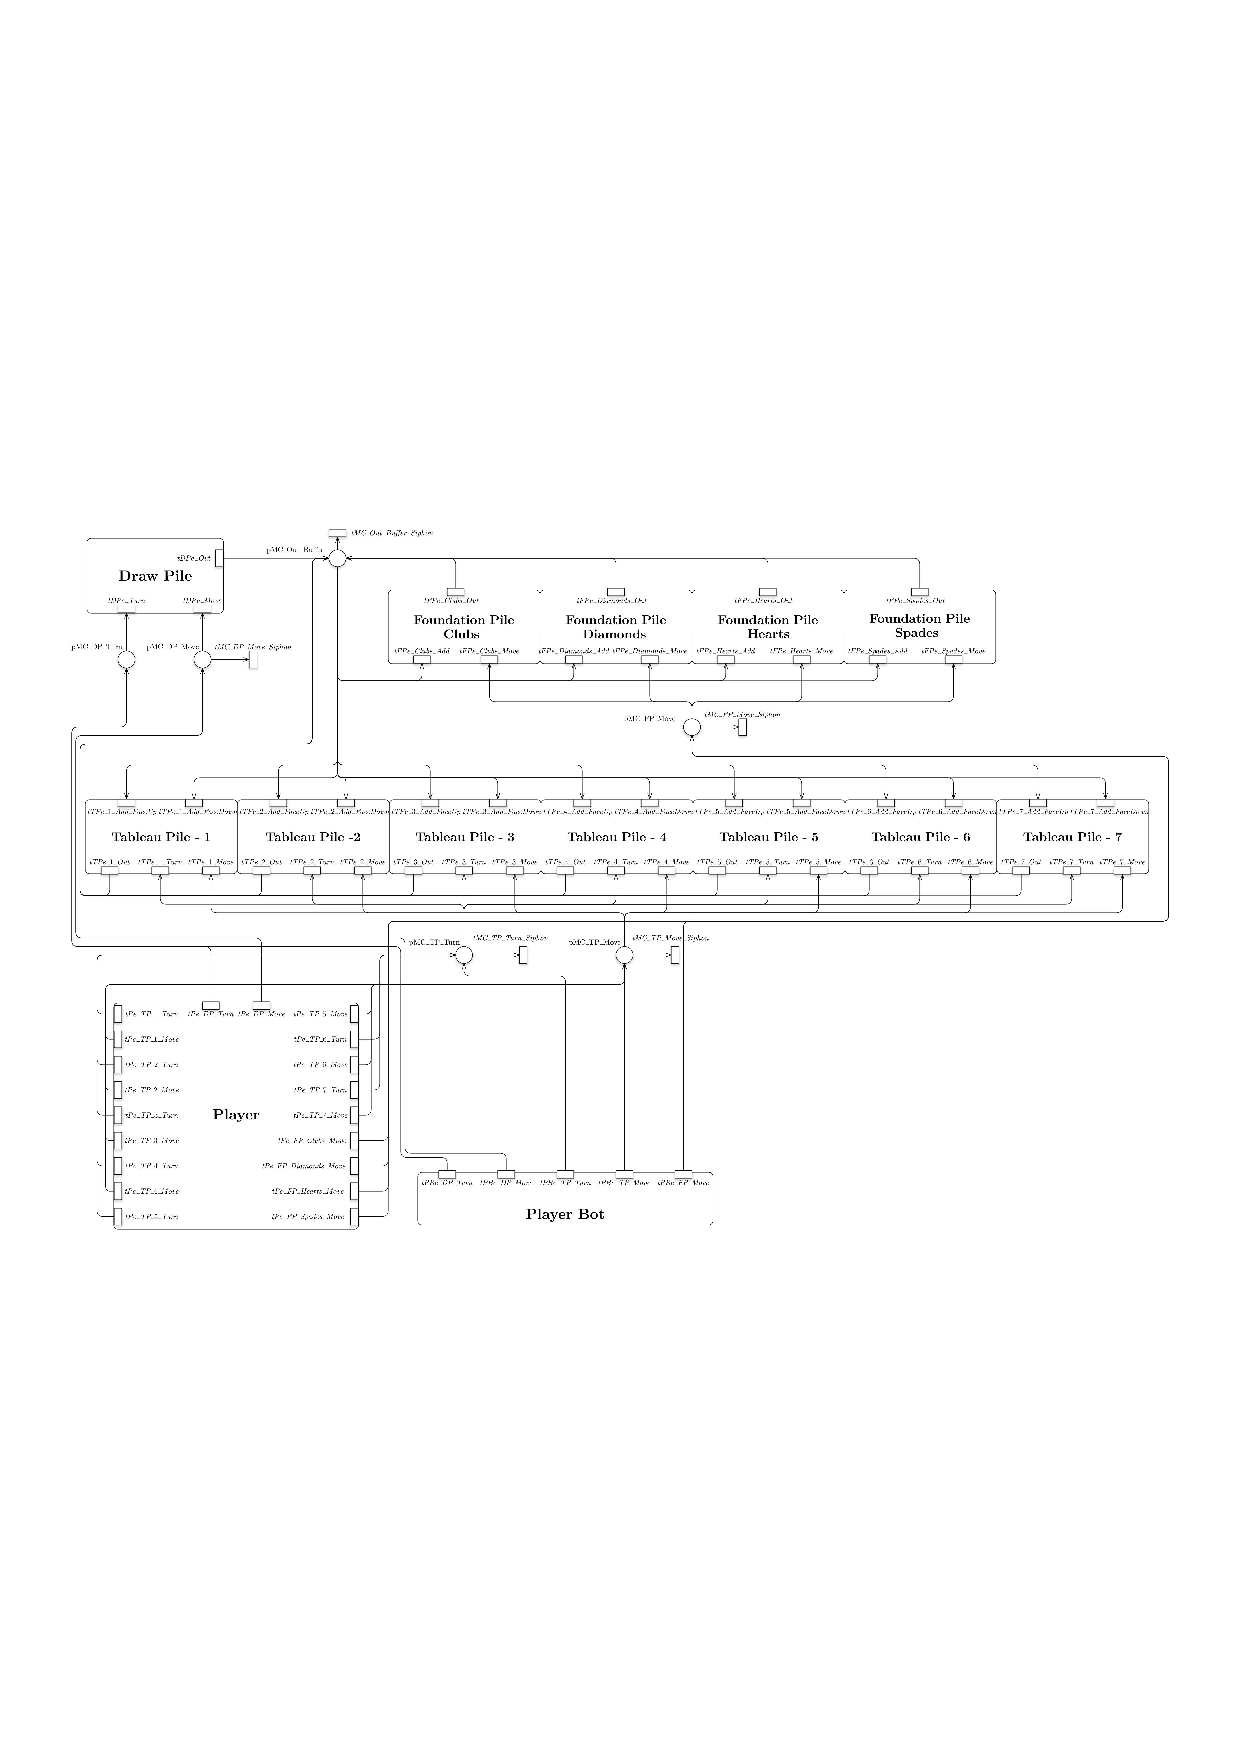
\includegraphics[trim=70 50 100 300,angle=90,scale=1.3]{images/overallViewPdf}
\end{center}
The model developed is pretty large, and contains 94 transition and 42 places. It is developed using the modualar approach, and encompasses 6 different modules. Some of the modules are duplicated, with the only difference being the names of the transitions and places.
\subsection{Draw Pile Module}
\begin{center}
	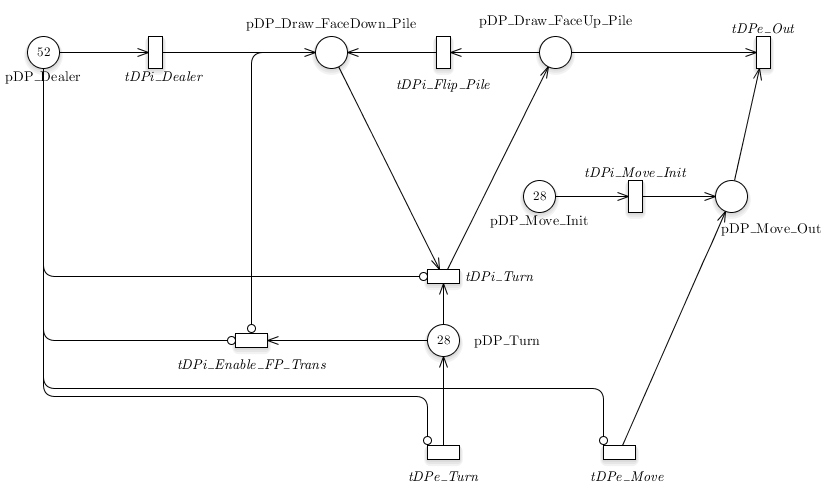
\includegraphics[width=\textwidth]{images/drawPile}
\end{center}
The Draw Pile module has several key responsibilities. When first running the model, it will use the initial tokens of \verb!pDP_Dealer! and give each of them a color according to the variable \verb!global_info.DECK!. If the \verb!global_info.RANDOM_DECK! is set, the cards are randomly dealt. 
\begin{table}
	\caption{Transitions used in Draw Pile}
	\begin{tabular}{|l|l|l|}
		\hline
		& Name & Description \\
		\hline
		1  & tDPe\_Move               &    \\ \hline
		2  & tDPe\_Out                &    \\ \hline
		3  & tDPe\_Turn               &    \\ \hline
		4  & tDPi\_Dealer             &    \\ \hline
		5  & tDPi\_Enable\_FP\_Trans  &    \\ \hline
		6  & tDPi\_Flip\_Pile         &    \\ \hline
		7  & tDPi\_Move\_Init         &    \\ \hline
		8  & tDPi\_Turn               &    \\ \hline
	\end{tabular}
\end{table}
\begin{table}
	\caption{Places used in Draw Pile}
	\begin{tabular}{|l|l|l|}
		\hline
		& Name & Description \\
		\hline
		1  & pDP\_Dealer               &  \\ \hline
		2  & pDP\_Draw\_FaceDown\_Pile &  \\ \hline
		3  & pDP\_Draw\_FaceUp\_Pile   &  \\ \hline
		4  & pDP\_Move\_Init           &  \\ \hline
		5  & pDP\_Move\_Out            &  \\ \hline
		6  & pDP\_Turn                 &  \\ \hline
	\end{tabular}
\end{table}
\subsection{Foundation Pile Module}
\begin{center}
	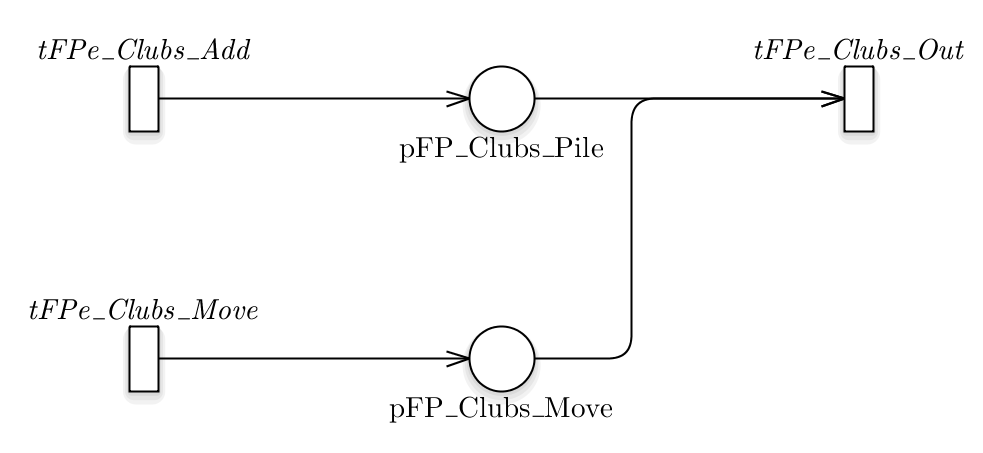
\includegraphics[width=\textwidth]{images/foundationPile}
\end{center}
\subsection{Tableau Pile Module}
\begin{center}
	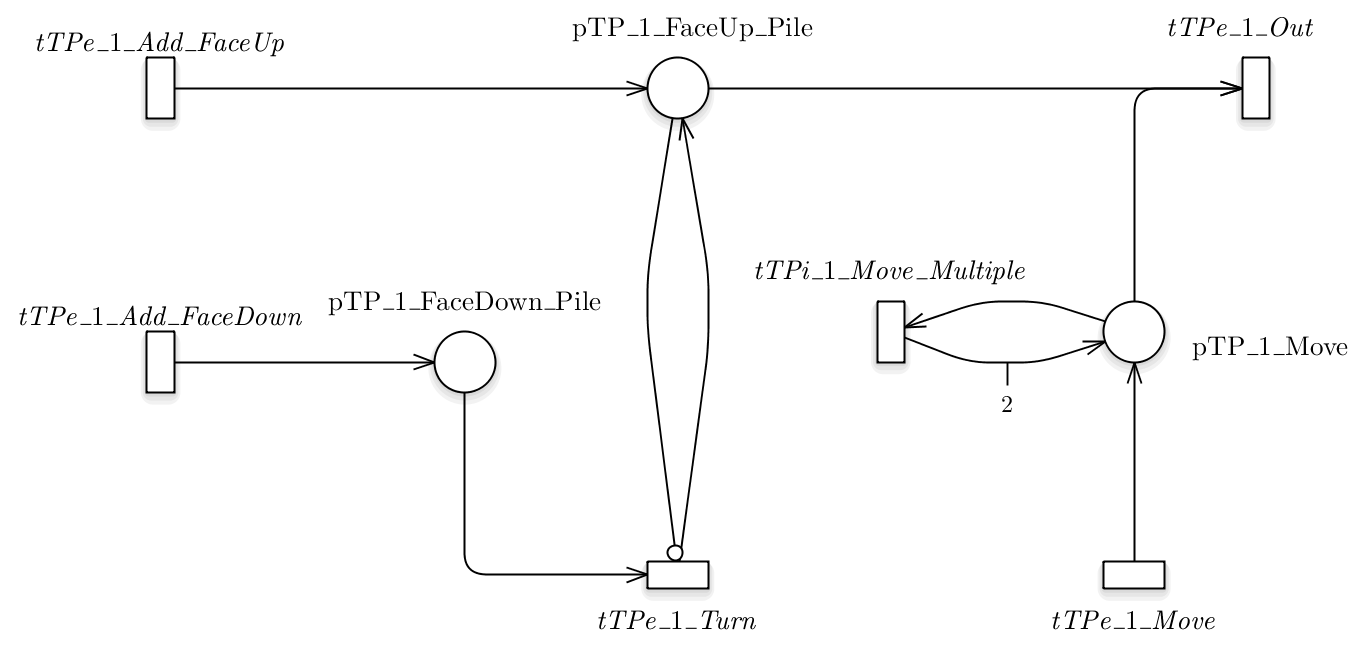
\includegraphics[width=\textwidth]{images/tableauPile}
\end{center}
\subsection{Module Connector Module}

\subsection{Player Module}

\subsection{Player Bot Module}


\section{Implementation}
\label{sec:3_implementation}
\subsection{Algorithms}
\subsubsection{Atomicity}
In order to preventdd
\subsection{Initial Dealing}
\subsection{Resources}
\subsection{Moving Multiple Cards}

\begin{verbatim}
    def mapper_from_to(self, key, email):
        if 'to' in email.keys() and 'from' in email.keys() and 'body_count' in email.keys():
\end{verbatim}

\section{Testing, Analysis and Results}
\label{sec:3_implementation}
\subsection{Algorithms}
\subsubsection{Atomicity}
In order to preventdd
\subsection{Initial Dealing}
\subsection{Resources}
\subsection{Moving Multiple Cards}

\section{Discussion}



% Keeping this for reference for now %
\begin{thebibliography}{7}

\bibitem{wikiTFIDF} Wikipedia article on Tf-idf. \url{https://en.wikipedia.org/wiki/Tf?idf}
\bibitem{oreilly} Tom White, Hadoop: The Definitive Guide, 2015, \emph{ISBN: 978-1-491-90163-2}
\bibitem{dockerdocs} Docker API Docs, \url{https://docs.docker.com}
\bibitem{dat630slides} Slides from DAT630, Krisztian Balog
\bibitem{dataset} Kaggle. The Enron Email Dataset. \url{https://www.kaggle.com/wcukierski/enron-email-dataset}
\bibitem{coursematerial} Data Intensive Systems Compendium, Tomasz Wiktorski et al.
\bibitem{git} Source code of all tasks developed. GitLab \url{https://gitlab.com/mindejulian/projectDAT500/tree/master}

\end{thebibliography}

\end{document}
